\documentclass[conference]{IEEEtran}
\usepackage{cite}
\usepackage{amsmath,amssymb,amsfonts}
\usepackage{algorithmic}
\usepackage{graphicx}
\usepackage[section]{placeins} % pone una barrera al final de cada sección/subsección
\usepackage{textcomp}
\usepackage[svgnames]{xcolor} % Listing background
\usepackage{svg}
% SVG rendering configuration (for IEEEtran + pdflatex)
\setsvg{
    inkscapelatex=false,
    width=\columnwidth,
    keepaspectratio
}
\usepackage{hyperref} % Cross-references are links
\usepackage{tabularx} % Add x word-wrap in table cells
\usepackage{listings} % Syntax highlighting
\usepackage{xcolor} % Listing background
\usepackage{flafter} % Figures after its reference in text
\usepackage[all]{nowidow} % Avoid widow lines
\usepackage{booktabs} % Horizontal lines in tables
\usepackage{float} % Add this in the preamble
\usepackage{comment}
\usepackage{tikz}
\usepackage{pgfplots}
\usepackage{balance} %IDO

\pgfplotsset{compat=1.18}
\usepackage{inconsolata} % Monospaced font

\def\BibTeX{{\rm B\kern-.05em{\sc i\kern-.025em b}\kern-.08em
    T\kern-.1667em\lower.7ex\hbox{E}\kern-.125emX}}

% Listing styles, see https://www.overleaf.com/learn/latex/Code_listing
\definecolor{codegreen}{rgb}{0,0.6,0}
\definecolor{codegray}{rgb}{0.5,0.5,0.5}
\definecolor{codepurple}{rgb}{0.58,0,0.82}
\definecolor{backcolour}{rgb}{0.97,0.97,0.95}

% See https://en.wikibooks.org/wiki/LaTeX/Source_Code_Listings#Settings
\lstdefinestyle{listing_style}{
    backgroundcolor=\color{backcolour},
    basicstyle=\ttfamily\footnotesize, % font family and size
    breakatwhitespace=true, % automatic breaks only at whitespace
    breaklines=true, % automatic line-breaking
    captionpos=b, % t=top, b=bottom
%   commentstyle=\color{codegreen},
    escapeinside={~[}{]~}, % Delimiters for Latex commands, eg: ~[\textbf{make test}]~
    frame=single, % none/leftline/topline/bottomline/lines/single/shadowbox
    keepspaces=true,
%   keywordstyle=\color{blue},
%   morekeywords={make,test,clean,asan,mkdir},
    numbers=left,
    numbersep=5pt, % distance of line-numbers from the code
    numberstyle=\tiny\color{codegray},
    rulecolor=\color{codegray}, % colour of the frame-box
%   showspaces=false,
%   showstringspaces=false,
%   showtabs=false,
%   stringstyle=\color{codepurple},
    tabsize=2
}

\lstset{style=listing_style}

% Adapted from https://tex.stackexchange.com/a/279134
\makeatletter
\def\ps@IEEEtitlepagestyle{%
  \def\@oddfoot{\mycopyrightnotice}%
  \def\@evenfoot{}%
}
\def\mycopyrightnotice{%
  {\footnotesize \hfill}
}
\makeatother

% Embed fonts for IEEE Pdf Express
% https://www.overleaf.com/learn/latex/Questions/My_submission_was_rejected_by_the_journal_because_%22Font_XYZ_is_not_embedded%22._What_can_I_do%3F

\begin{document}

\title{Performance Evaluation of Asynchronous I/O and Parallel Execution Strategies in Relational Databases}

\newif\ifanonymous
\anonymoustrue % Enable this line for blind review

\newcommand{\AnonymousAuthor}{%
\IEEEauthorblockN{Anonymous Author}
\IEEEauthorblockA{\textit{Department} \\
\textit{Affiliation}\\
Address \\
email@address}
}

\author{
\ifanonymous

\AnonymousAuthor\and
\AnonymousAuthor\and
\AnonymousAuthor\and
\AnonymousAuthor

\else
\IEEEauthorblockN{Archibald Carrion-Claeys}
\IEEEauthorblockA{\textit{ECCI} \\
\textit{Universidad de Costa Rica}\\
San José, Costa Rica \\
archibald.carrion@ucr.ac.cr}
\and
\IEEEauthorblockN{Francisco Ulate-Alpízar}
\IEEEauthorblockA{\textit{ECCI} \\
\textit{Universidad de Costa Rica}\\
San José, Costa Rica \\
francisco.ulate@ucr.ac.cr}
\and
\IEEEauthorblockN{Ignacio Diaz-Oreiro}
\IEEEauthorblockA{\textit{ECCI} \\
\textit{Universidad de Costa Rica}\\
San José, Costa Rica \\
ignacio.diazoreiro@ucr.ac.cr}
\and
\IEEEauthorblockN{Jeisson Hidalgo-Céspedes}
\IEEEauthorblockA{\textit{ECCI-CITIC} \\
\textit{Universidad de Costa Rica}\\
San José, Costa Rica \\
jeisson.hidalgo@ucr.ac.cr}
\fi
}


\maketitle

\begin{abstract}
Modern database management systems rely on efficient input/output strategies to handle large and diverse workloads. This study focused on PostgreSQL, in which the asynchronous method was introduced in version 18. Many engines still use synchronous I/O. Nevertheless, the implementation of asynchronous and parallel methodologies suggests a significant reduction in latency for demanding workloads. Parallel I/O workers and the Linux \texttt{io\_uring} asynchronous interface could improve query performance, in particular for read-intensive loads. However, their practical benefits across diverse workload patterns remain underexplored in the scientific literature. Our study compared the performance of PostgreSQL~18, configured in three I/O modes (synchronous, background workers, and \texttt{io\_uring}).
This study addressed a fundamental question: to what extent do asynchronous I/O and parallel execution strategies improve query performance compared to traditional single-threaded synchronous I/O in relational databases? We systematically compared three I/O approaches in PostgreSQL 18: (1) single-threaded synchronous I/O (baseline), (2) background workers (parallel synchronous I/O across multiple threads), and (3) io\_uring (true asynchronous I/O with non-blocking submission). Using TPC-H benchmarks at three scales (100MB, 1GB, and 10 GB), we measured query execution time across 22 read-intensive analytical queries under controlled conditions. The experiment was conducted on a virtualized environment on a blade server. This environment represents a realistic production deployments.
%The fundamental research questions are (1) to what extent are asynchronous I/O models more efficient than traditional blocking I/O models in database systems? and (2) what are the performance trade-offs when implementing asynchronous I/O for both read-intensive and write-intensive operations?
%We used a benchmark suite based on the TPC-H standard and a dataset of at least 40~GB. With experiments conducted under both cold starts (empty buffer cache) and warm buffers. The evaluation focuses primarily on read-intensive queries. However, additional write and mixed workloads are included to observe behavioral trade-offs in more realistic environments. To understand the performance trade-offs, we analyzed query latency and throughput, correlating them with I/O wait states to pinpoint efficiency gains. 
% should we add information about the hardware used for the tests?
The asynchronous I/O models did outperform traditional synchronous I/O in PostgreSQL 18, in particular for read-intensive workload. However, the performance gains did vary based on workload patterns, with a variety of read pattern being the one with less performance improvement, and read-only pattern with the most gains.
\end{abstract}

\begin{IEEEkeywords}
 PostgreSQL, io\_uring, asynchronous I/O, database performance, benchmarking
\end{IEEEkeywords}



\section{Introduction}
\label{sec:Introduction}

Contemporary relational database systems face fundamental scalability challenges. These systems must maintain performance integrity while accommodating increasing numbers of simultaneous database transactions and growing user demands~\cite{silva_towards_2015}.
The foundational work on IBM System R established that disk access costs typically dominate query execution time, making access path optimization critical for database performance~\cite{selinger_access_1979}.
Input/output operations have long been recognized as a primary bottleneck in database performance, particularly for storage-bound workloads, where the cost formula explicitly weights page fetches as the dominant factor over CPU utilization~\cite{selinger_access_1979}.
Traditional synchronous I/O models require blocking-based operations, whereas asynchronous I/O does not~\cite{pestka2024aio}. 
%The emphasis on minimizing "total access cost" in early database optimizers reflects the fundamental understanding that I/O efficiency determines overall system performance~\cite{selinger_access_1979}.
The historical limitations of POSIX asynchronous I/O, which Axboe described as "lackluster"  with poor performance~\cite{axboe2019io_uring}, motivated the development of more efficient alternatives like io\_uring which we evaluated in this study.
Recent developments in operating system interfaces, like Linux's io\_uring~\cite{An2024A2L}, addressed these I/O limitations through asynchronous mechanisms. Database systems also offered opportunities to address this issue~\cite{do_need_1999}.
PostgreSQL 18 introduced support for asynchronous I/O through background workers and io\_uring integration. PostgreSQL 18 provided a practical testbed for evaluating these approaches against conventional synchronous operations. % While asynchronous I/O promises to reduce context switching overhead \cite{pestka2024aio} and improve resource utilization through I/O-compute overlap, it seems that the empirical performance benefits across varying workload characteristics remain not fully understood \cite{chen_uring_2025}.

%This study compares three I/O configurations—synchronous, background workers, and io\_uring—using TPC-H-based benchmarks focused on read-intensive workloads. At the time of the writting of this article, PostgreSQL do not support asynchronous write operation, only asynchronous read operations. Our research question addresses whether asynchronous I/O access modes provide performance improvements over synchronous I/O for read-heavy database operations.
This study addressed a fundamental question: \emph{To what extent do asynchronous I/O mechanisms and parallel execution strategies improve query performance compared to traditional single-threaded synchronous I/O in modern relational databases?} Specifically, we compared three I/O approaches in PostgreSQL 18: (1) synchronous blocking I/O (single-threaded baseline), (2) background workers (parallel synchronous I/O across multiple threads), and (3) io\_uring (true asynchronous I/O with non-blocking submission)—quantifying performance gains across varying database scales using TPC-H benchmarks focused on read-intensive workloads. Performance improvements are defined as reductions in query execution time while maintaining equivalent result accuracy.

Our study focused specifically on read-intensive operations, as PostgreSQL 18's asynchronous I/O support is currently limited to read operations, with write operations remaining synchronous. We selected PostgreSQL~18 as it supports three distinct I/O methodologies (synchronous, workers, and io\_uring) within a single code base at the time of writing. This enabled controlled comparison while eliminating confounding variables.

Alternative database management systems such as MySQL, Oracle, and SQL Server either lack asynchronous support or uses an older implementation. \begin{comment}
    which could introduce architectural differences confounding I/O performance isolation.
\end{comment}
PostgreSQL's configurable I/O subsystem enables isolation of I/O methodology effects while maintaining identical query processing and execution environments across all experimental conditions.


\section{Theoretical framework}
\label{sec:theoreticalframework}

This section establishes the core concepts necessary to analyze and compare synchronous, parallel, and asynchronous I/O methods in database systems. It begins by introducing workload patterns and the TPC-H benchmark. IOt then details the specific I/O methods available in PostgreSQL that form the basis of our experimental comparison.

Also, we introduced some concepts like workload patterns, the benchmark TPC, and its model tpc-h for the analysis of the performance affecting both asynchronous and synchronous operations.

\begin{comment}
    
Fig.~\ref{fig:three_io_methods_1} illustrates the three I/O approaches evaluated in this study: synchronous I/O, background workers, and io\_uring.

% Estaba three_io_methods.png
\begin{figure}[htbp]
    \centering
     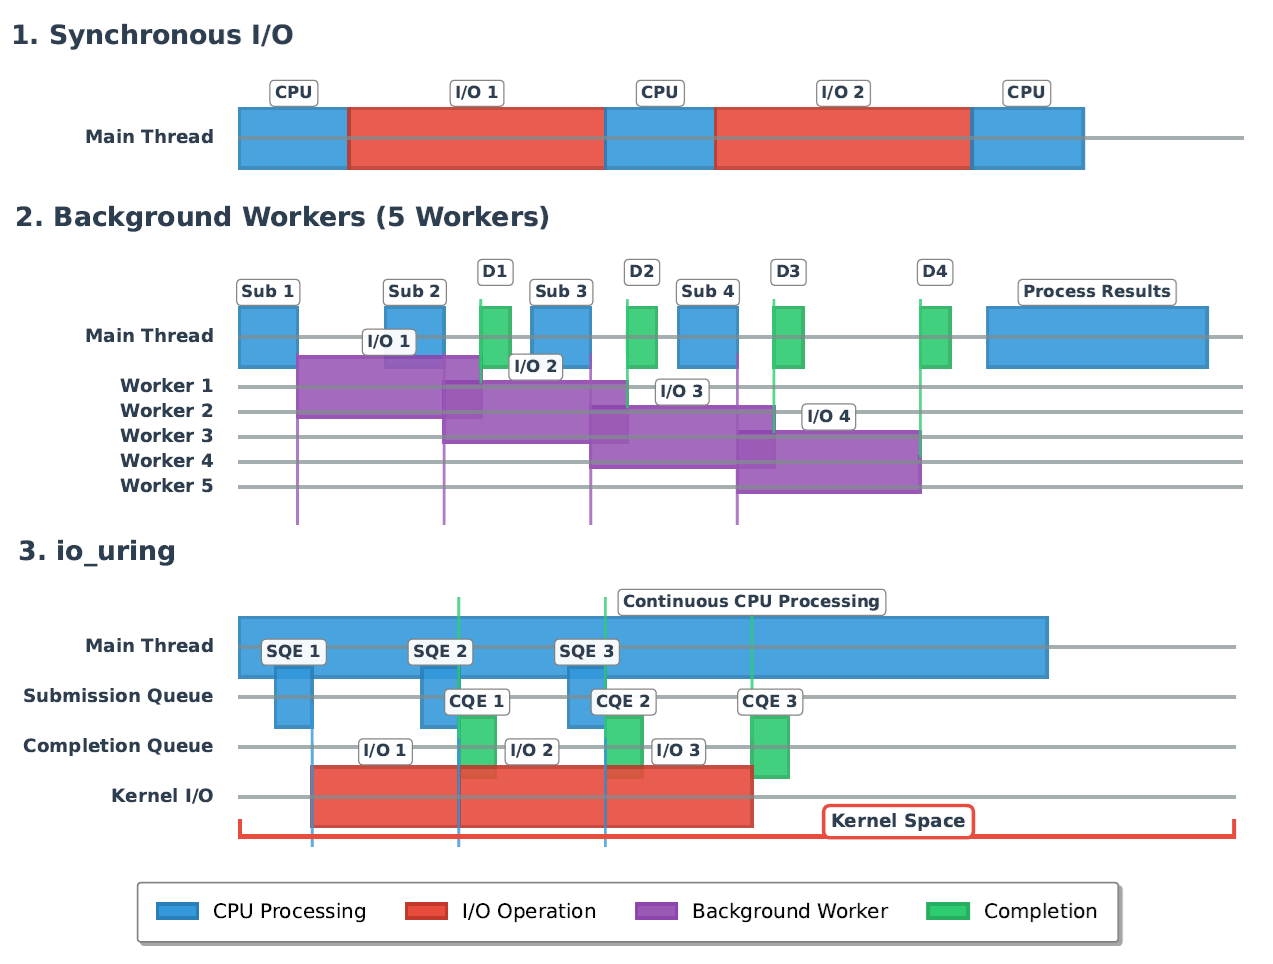
\includegraphics[width=\columnwidth]{images/three_io_methods_id2.png}
    \caption{Comparison of three I/O processing methods: (1) Synchronous I/O blocks the main thread during each operation, (2) Background workers offload I/O to separate threads while the main thread coordinates, and (3) io\_uring enables continuous CPU processing through submission and completion queues with kernel-space I/O handling.}
    \label{fig:three_io_methods_1}
\end{figure}
\end{comment}


\subsection{Workload Patterns and Performance Characteristics}
\label{subsec:workload_patterns}

The efficiency of an I/O strategy is highly dependent on the nature of the database workload~\cite{An2024A2L}. We categorized workloads based on their access patterns, as these patterns directly influenced whether I/O becomes a bottleneck in:

\begin{itemize}
\item \textbf{OLTP (Online Transaction Processing)} systems are characterized by short, frequent read and write operations, such as inserts and updates. These systems prioritize low-latency response times and robust concurrency control~\cite{Chaudhuri1997}.
\item \textbf{OLAP (Online Analytical Processing)} systems are designed to execute complex queries over large volumes of historical data. In this context, maximizing \textbf{query throughput} is the primary performance objective~\cite{Chaudhuri1997}.
\end{itemize}

OLAP workloads are inherently I/O-bound, as they typically require full or partial scans of large datasets~\cite{Sirin2020}. This characteristic makes them particularly sensitive to the efficiency of the underlying I/O subsystem. 
\begin{comment}    
, a bottleneck exacerbated by the significant performance gap between modern CPUs and storage media~\cite{tanenbaum_structured_2013}. 
\end{comment}


\subsection{TPC-H Benchmark}
\label{subsec:TPC-H-benchmarks}

To measure efficiency this study employed the TPC-H benchmark, a widely recognized \emph{decision-support benchmark}. TPC-H models an OLAP-like environment with an eight-table schema and a scalable data generator (DBGEN). It specifies 22 business-oriented, read-only queries that stress database operations through complex scans, joins, and aggregations~\cite{TPC-H-3.0.1}.

The TPC-H schema represents a simplified retail business scenario with tables modeling parts, suppliers, customers, orders, and geographic hierarchies. Figure~\ref{fig:tpch_schema} illustrates the relationships between these entities, where the LINEITEM table serves as the central fact table connecting orders with their constituent parts and suppliers.
The schema's cardinalities range from small dimension tables (REGION with 5 rows, NATION with 25 rows) to large fact tables (LINEITEM with approximately 6 million rows at scale factor 1), enabling realistic testing of query optimization and join strategies across varied data volumes.

\begin{figure}[htbp]
    \centering
     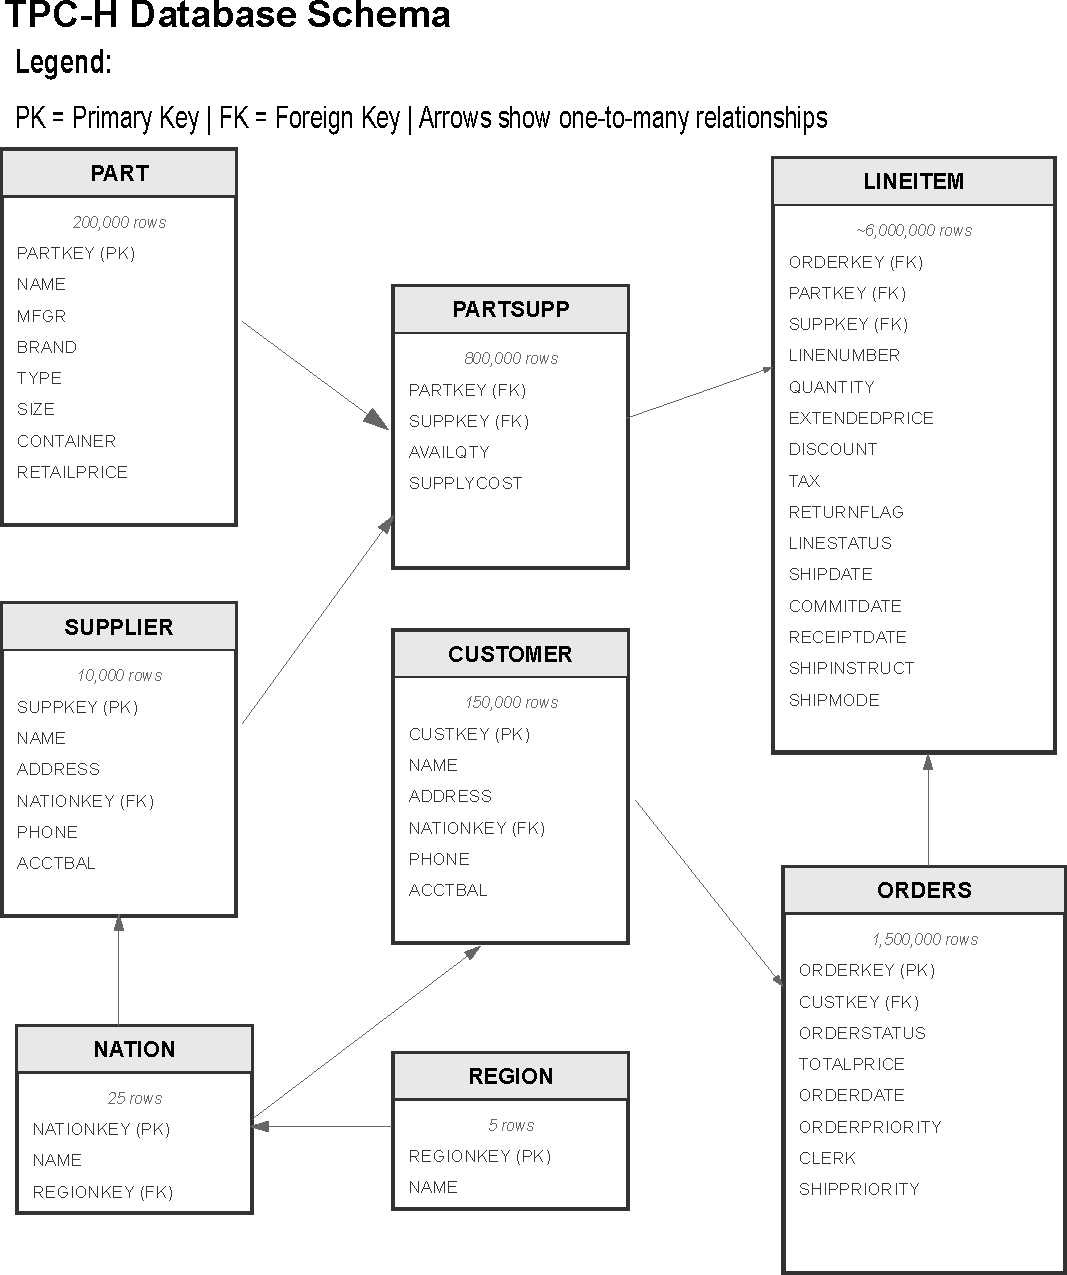
\includegraphics[width=\columnwidth]{images/tpch_schemat.pdf}
    \caption{TPC-H database schema.}
    \label{fig:tpch_schema}
\end{figure}

A fully compliant TPC-H execution involves two primary tests: the Power test (focused on single-stream performance) and the Throughput test (measuring concurrent query execution). The benchmark's official metric, QphH@Size, is a composite of these tests, representing queries per hour at a specified data scale~\cite{TPC-H-3.0.1}.

\subsection{PostgreSQL I/O methods: synchronous, workers, and io\_uring}
\label{subsec:3_methods}

The selection of PostgreSQL for this evaluation is strategic: it offered configurable I/O methods within a single, consistent code-base, enabling direct comparison without the confounding variables that would arise from comparing different database systems. This allowed us to isolate the effects of I/O methodology while maintaining identical query processing, optimization, and execution environments.

PostgreSQL 18 introduced configurable I/O methods which defined how the database engine interacted with the operating system to perform disk reads. These modes—\texttt{synchronous}, \texttt{worker}, and \texttt{io\_uring}—represented three different ways of handling I/O concurrency. Figure~\ref{fig:three_io_methods_2} illustrate the fundamental differences between these approaches.

\begin{figure}[htbp]
    \centering
     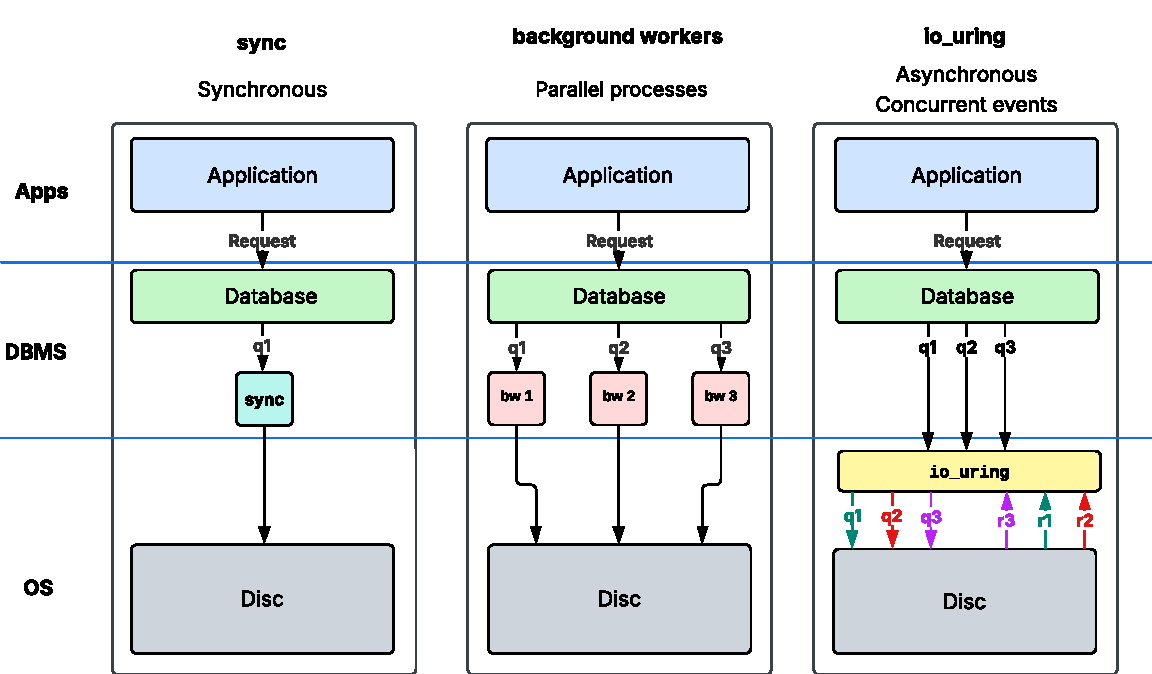
\includegraphics[width=\columnwidth]{images/comparative_input_settings.pdf}
    \caption{Side by side comparison of three I/O processing methods.}
    \label{fig:three_io_methods_2}
\end{figure}

\paragraph{Synchronous I/O (\texttt{sync})}
In the \texttt{synchronous method} there is only one thread which stays idle while waiting for the answer from storage. The thread cannot proceed until it gets the requested data, which makes it simple and predictable.

\paragraph{Background workers (\texttt{worker})}
To overcome the blocking behavior of \texttt{synchronous method}, PostgreSQL can use background I/O workers. These helper threads handle read operations, allowing the main thread to schedule several reads and perform computations or prepare further requests while others complete.


\paragraph{io\_uring}
The \texttt{io\_uring} API, introduced in Linux 5.1, allows user-space applications to submit I/O operations directly through shared submission queue (SQ) and completion queue (CQ) mapped between user space and kernel space. PostgreSQL leveraged this mechanism to queue multiple read requests at once.

Each approach offered a trade-off. \texttt{Synchronous} prioritizes simplicity. \texttt{Worker} enables synchronous parallelism while using similar implementation to synchronous. \texttt{Io\_uring} offers an asynchronous implementation methods by letting user space and the kernel cooperate more closely.

\begin{comment}    
The figures~\ref{fig:iouring-overview} and~\ref{fig:iouring-detail} show in details the inner working of io\_uring.
In our experiments, these implementations corresponded to the configurations compared in Section~\ref{sec:Methodology}.
\end{comment}

\begin{comment}
\begin{figure}[htbp]
    \centering
    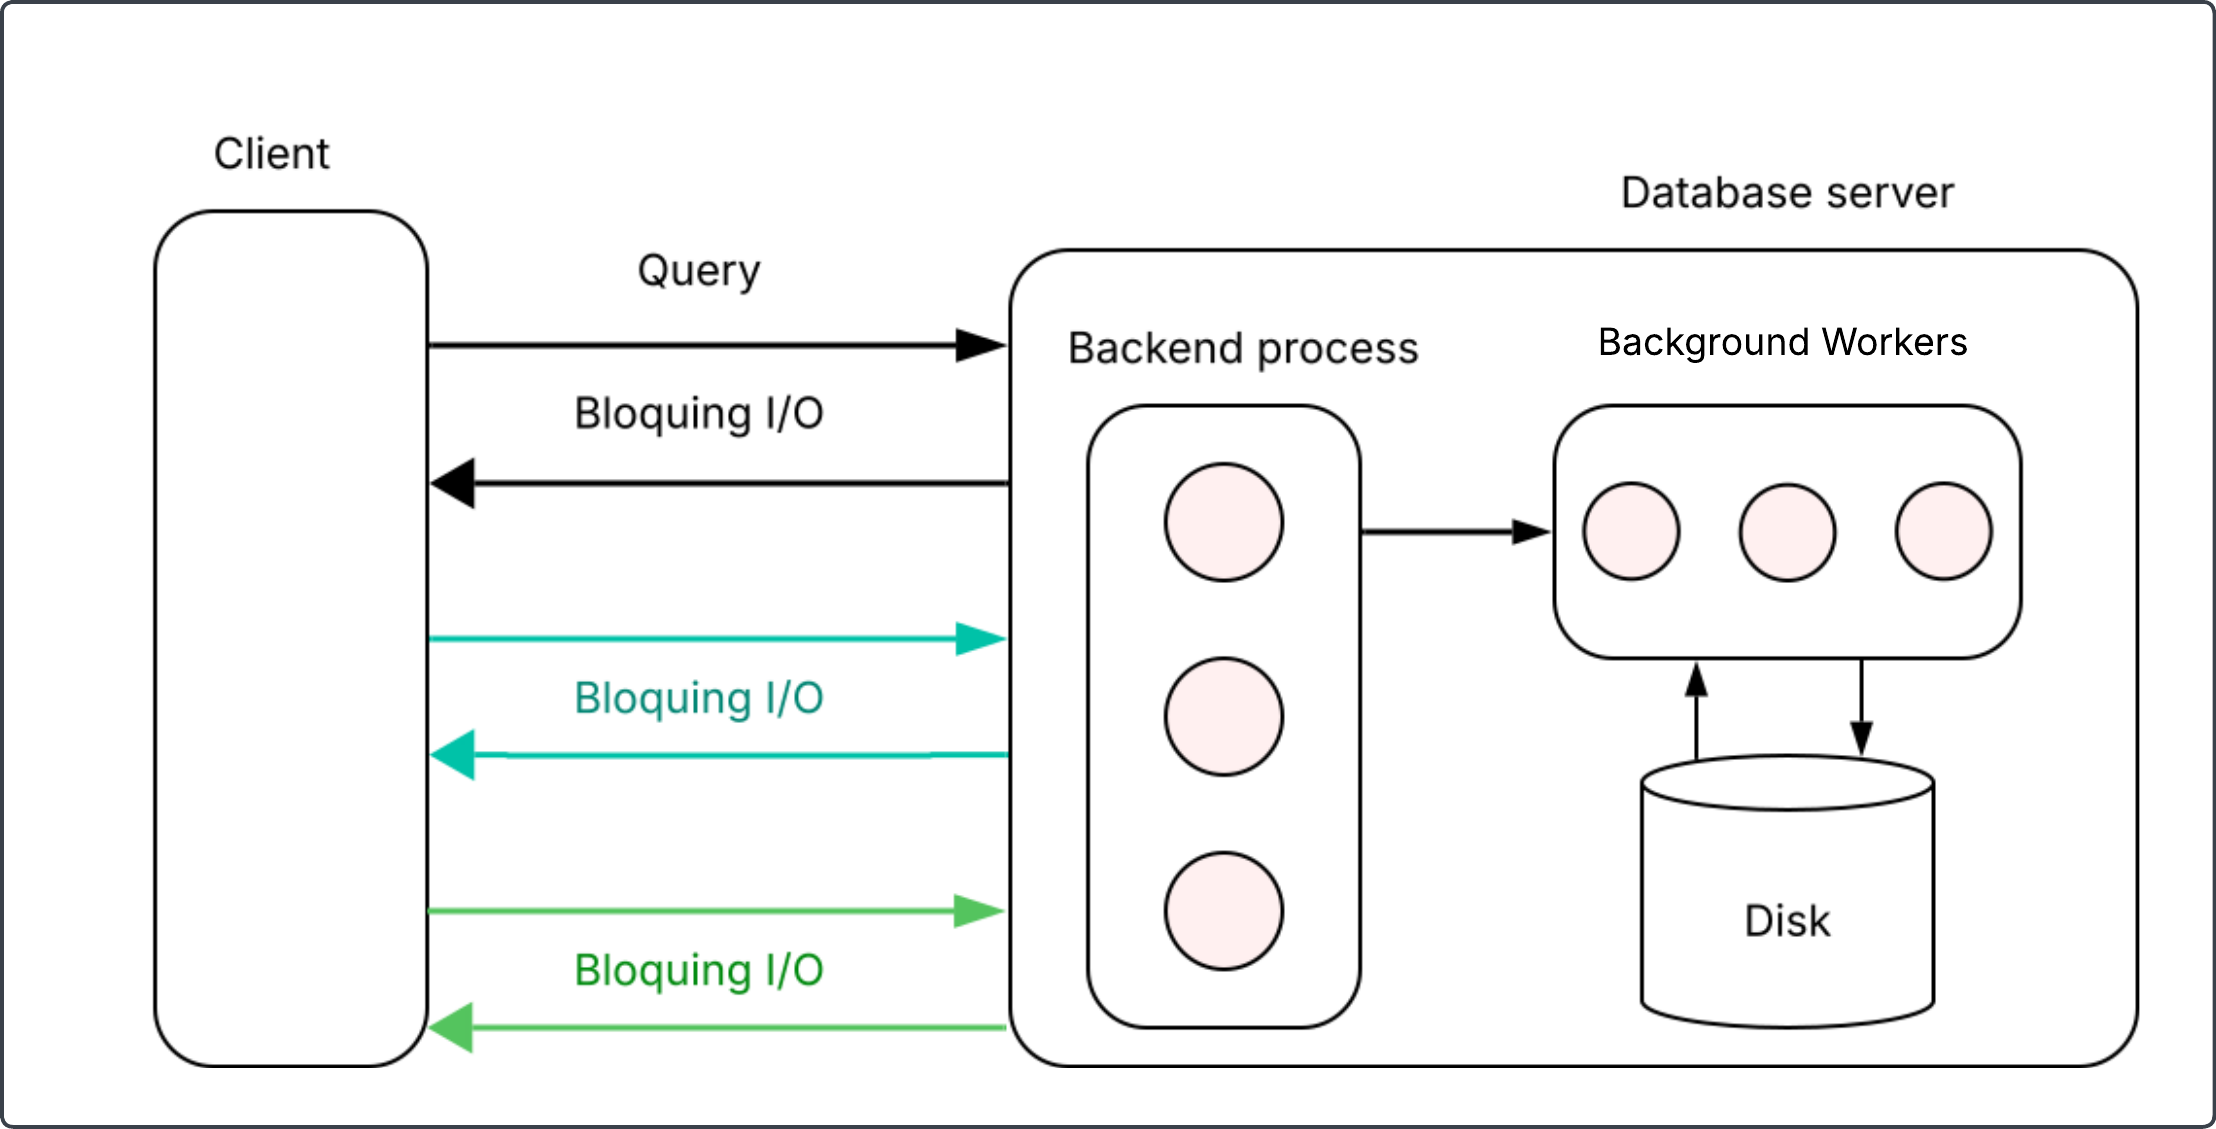
\includegraphics[width=\columnwidth,keepaspectratio]{images/workers}
    \caption{Background I/O workers: the backend process submits read requests to worker processes, which perform the actual disk access and return results asynchronously.}
    \label{fig:bgworkers}
\end{figure}
\end{comment}

\begin{comment}
    
\begin{figure}[htbp]
    \centering
    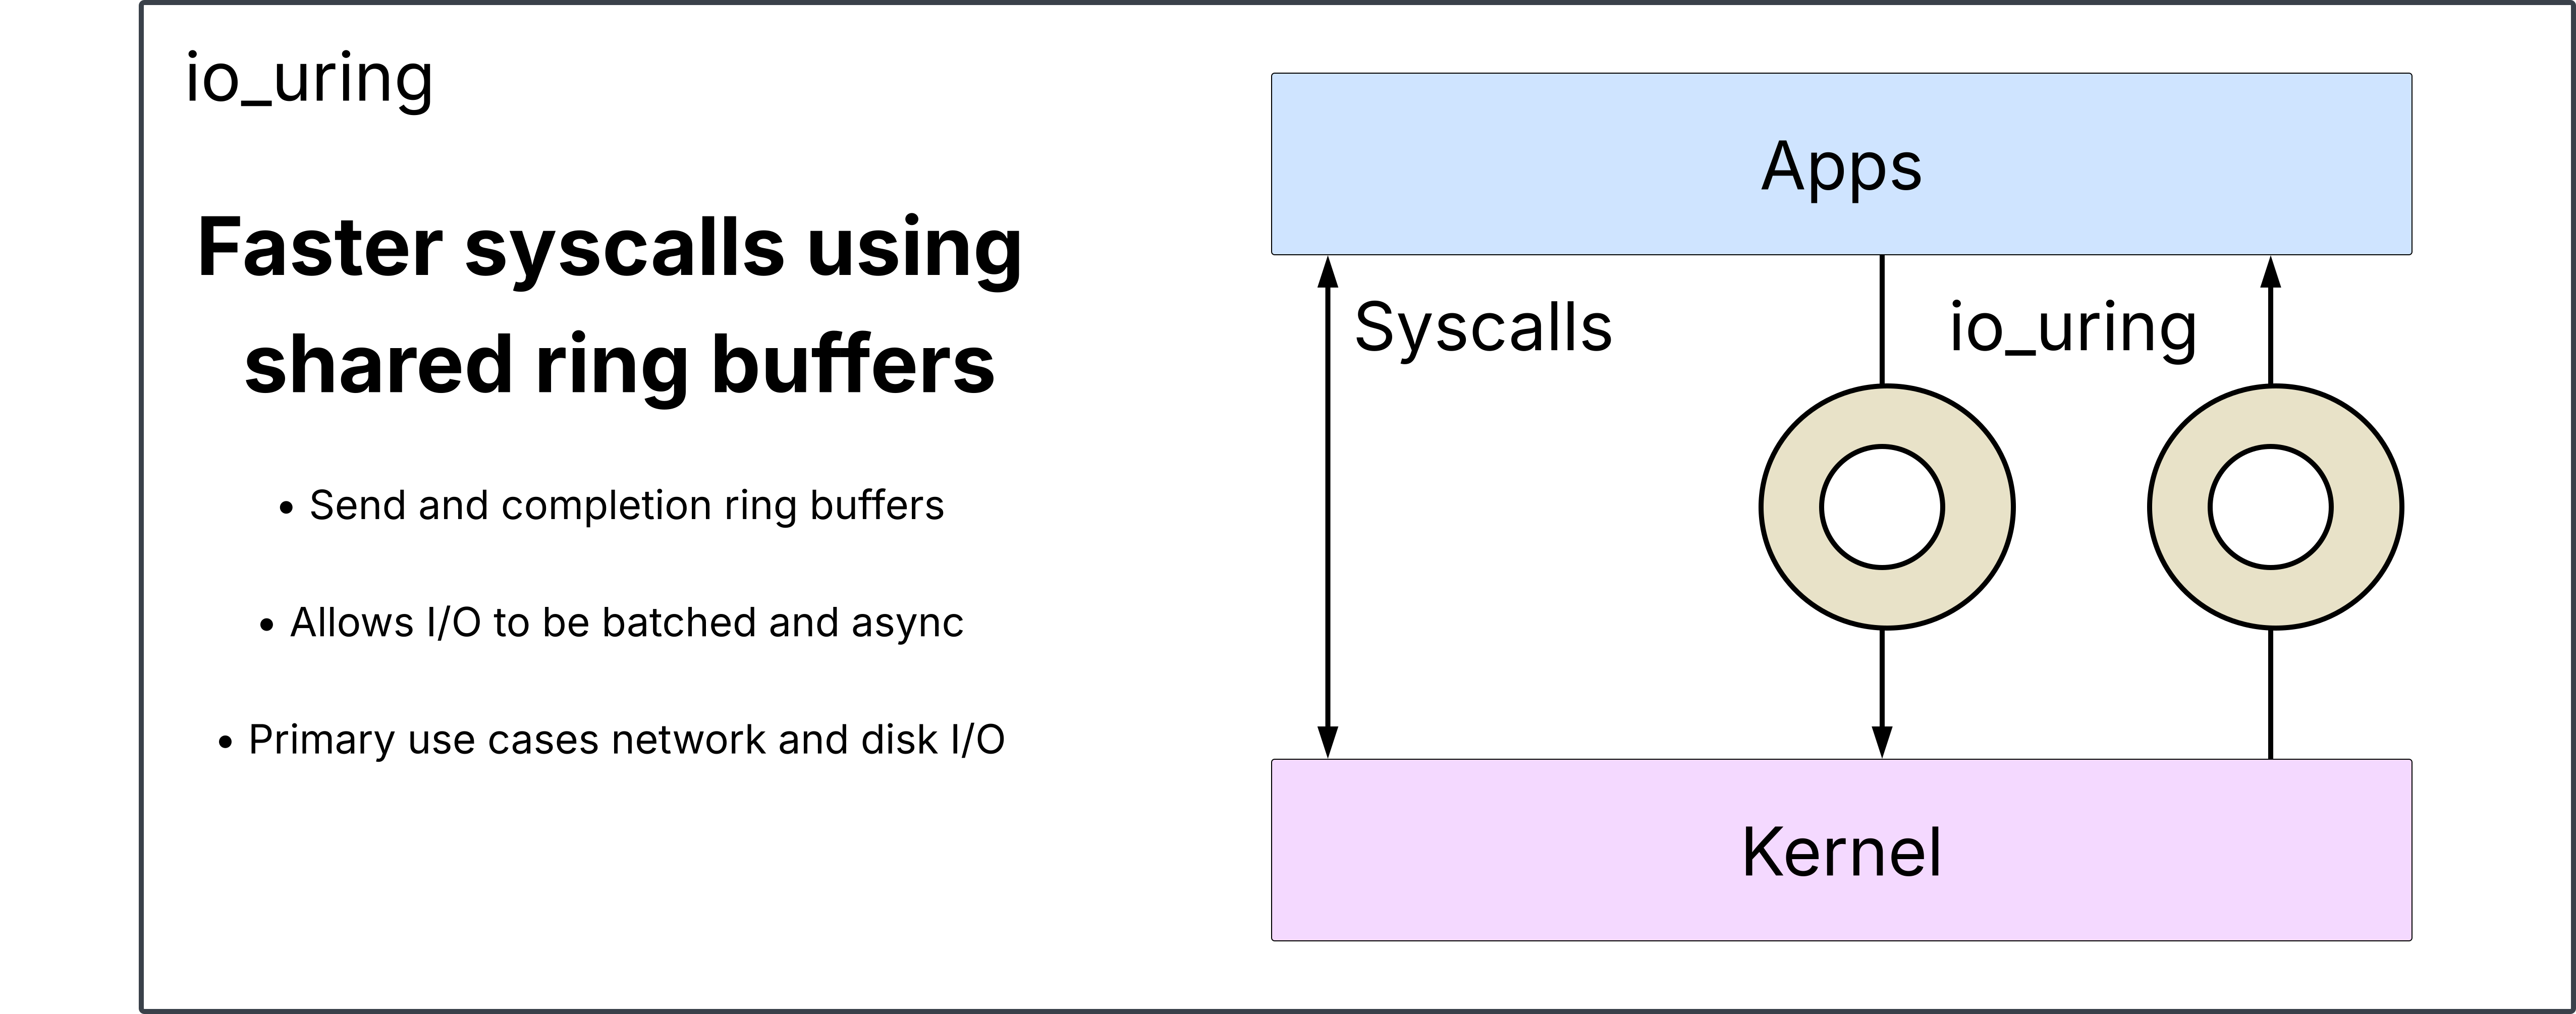
\includegraphics[width=\columnwidth,keepaspectratio]{images/io_uring}
    \caption{\texttt{io\_uring} overview: deep queues and batching help PostgreSQL overlap computation with storage latency, minimizing idle time and system calls.}
    \label{fig:iouring-overview}
\end{figure}

\begin{figure}[htbp]
    \centering
    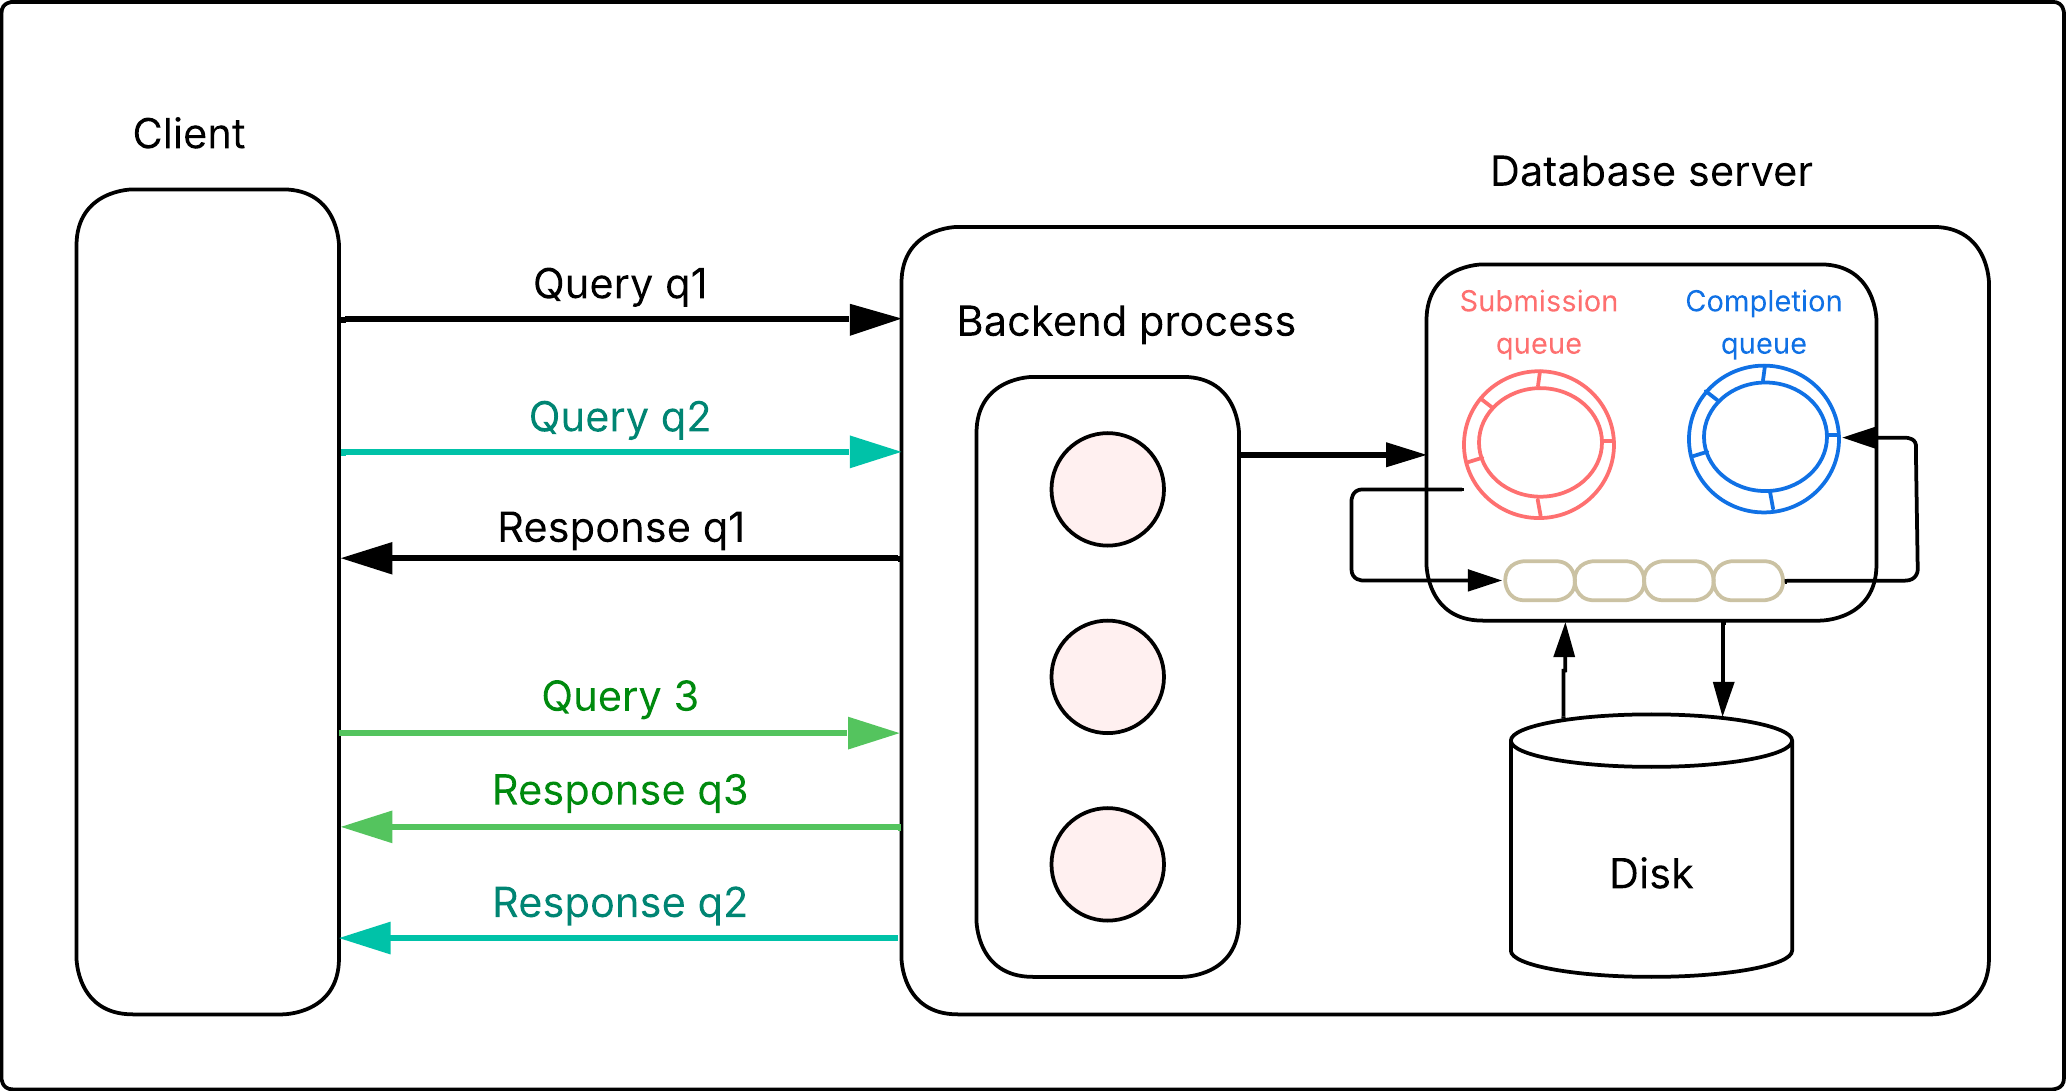
\includegraphics[width=\columnwidth,keepaspectratio]{images/io_uring_great}
    \caption{\texttt{io\_uring} in detail: user space submits multiple read operations via a shared submission queue, while the kernel asynchronously completes them and posts results to the completion queue.}
    \label{fig:iouring-detail}
\end{figure}
\FloatBarrier
\end{comment}

\section{Previous Work}
\label{sec:PreviousWork}
To identify studies evaluating the performance of synchronous versus asynchronous I/O in relational database systems, we conducted a structured literature review illustrated in the figure~\ref{fig:literature_review}. We focused on performance comparison under different database size, and, most important for our investigation, read method. We performed an initial keyword-based search in the Scopus database using the following queries \texttt{"asynchronous I/O" AND database} OR \texttt{io\_uring} OR \texttt{PostgreSQL AND "database performance" AND ("I/O workers" OR "background worker")}. To find more related publications we used backward and forward snowballing, this way we obtained 9 investigation which we found of value for our investigation.

Table~\ref{tab:tools} shows the following characteristics relevant to our research question: the database system used, whether it compared synchronous and parallel I/O modes, the hardware platform, database size and the primary evaluation metric. The table presents the studies in chronological order, from the earliest work on io\_uring in 2019 to our current study in 2025, providing a temporal perspective on the evolution of asynchronous I/O research in database systems.

\begin{comment}
Table~\ref{tab:tools} shows the following characteristics relevant to our research question: the database system used, whether it compared synchronous and parallel I/O modes, the hardware platform, database size and the primary evaluation metric. The table presents the characteristics in a logical order aligned with our research focus on I/O performance comparison across different environments.
\end{comment}

\begin{table*}[h]
    \centering
    \caption{Summary of Asynchronous I/O Techniques in Database Systems}
    \begin{tabularx}{\textwidth}{l l l l l l X}
    \toprule
    \textbf{Study} & \textbf{Date} & \textbf{Database System} & \textbf{Async vs Sync} & \textbf{Hardware Platform} & \textbf{Database Size} & \textbf{Primary Evaluation Metric} \\
    \midrule
    Axboe~\cite{axboe2019io_uring} & 2019 & io\_uring design & Async only & Linux kernel & N/A & I/O performance, CPU overhead \\
    Mehdi et al.~\cite{Mehdi2023ScaleDB} & Jul 2023 & ScaleDB (in-memory) & Async only & Multi-core servers & In-memory & Throughput (QPS/TPS), Abort rate \\
    Pestka et al.~\cite{pestka2024aio} & Nov 2024 & Theoretical analysis & Async only & Modern SSDs & N/A & IOPS scaling, CPU sensitivity \\
    Chen et al.~\cite{chen_uring_2025} & Nov 2024 & Redis (in-memory) & Async only & Ryzen 7 + NVMe & In-memory datasets & Throughput (ops/s), Persistence time \\
    Xiao et al.~\cite{xiao_breaking_2025} & Jul 2025 & FlashANNS (ANNS) & Async only & NVMe SSD & Billion-scale vectors & Throughput (QPS), Recall \\
    \textbf{Our Study} & \textbf{2025} & \textbf{PostgreSQL 18} & \textbf{Both compared} & \textbf{VM} & \textbf{100MB-10GB} & \textbf{TPC-H metrics (Query execution time)} \\
    \midrule
    \end{tabularx}
    \label{tab:tools}
\end{table*}

\begin{figure}[htbp]
    \centering
     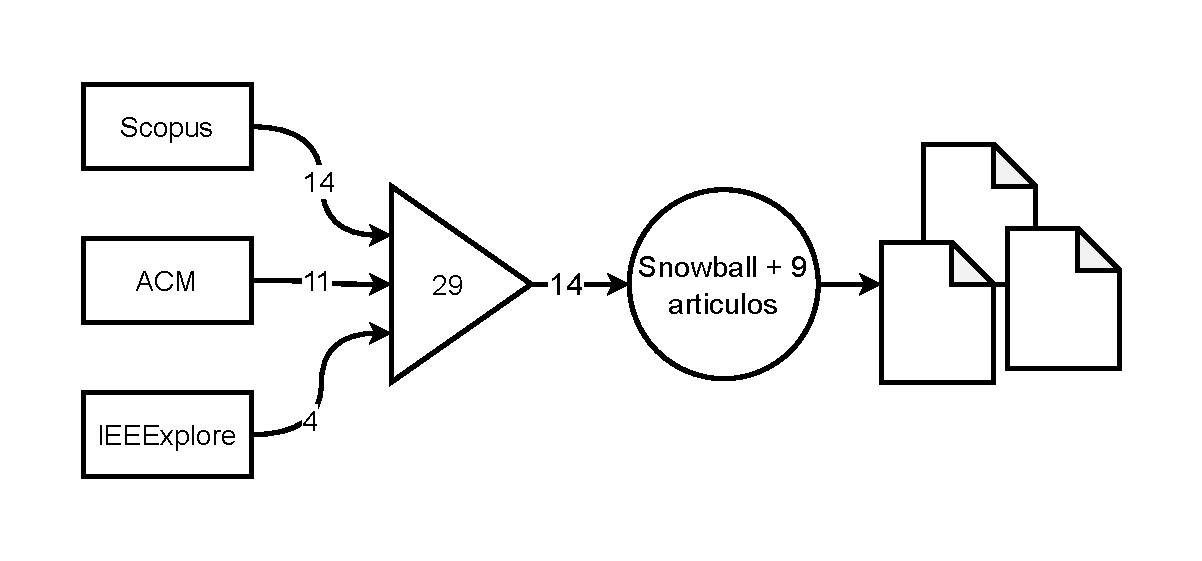
\includegraphics[width=\columnwidth]{images/literature_roadmap.pdf}
    \caption{Methods used to find our literature.}
    \label{fig:literature_review}
\end{figure}


In 2019, Axboe introduced io\_uring as a new approach to asynchronous I/O in Linux, addressing limitations of previous interfaces like AIO~\cite{axboe2019io_uring}. This work provided the architectural foundation for PostgreSQL's io\_uring implementation that we evaluated.

In July 2023, Mehdi et al. introduced ScaleDB, showing how asynchronous range-index updates can unlock scalability in environments where synchronous approaches collapsed under contention~\cite{Mehdi2023ScaleDB}. Their work showed that asynchronous concurrency control mechanisms can significantly improve throughput in high-contention scenarios.

In November 2024, Pestka et al. provided a theoretical foundation for asynchronous I/O, explaining why traditional blocking I/O becomes problematic on modern storage hardware and why adoption of those asynchronous implementation in production databases has been slow despite potential benefits~\cite{pestka2024aio}.

Also in November 2024, Chen et al. explored \texttt{io\_uring} for Redis persistence. They found that a synchronous I/O provides the most benefit for medium to large payload sizes in disk-bound scenarios~\cite{chen_uring_2025}. This workload-dependent performance improvement informs our expectation that database scale may similarly affects the benefits of asynchronous I/O in PostgreSQL.

In July 2025, Xiao et al. demonstrated that asynchronous I/O scheduling can dramatically improve throughput in data-intensive applications by effectively overlapping storage access with computation~\cite{xiao_breaking_2025}. While focused on approximate nearest search, their work illustrates the fundamental principle that drives our research: decoupling I/O from computation can break storage-compute bottleneck.

Collectively, these studies establish that asynchronous I/O can provide significant performance improvements, but the benefits are context-dependent and implementation-challenging. However, none of the previously mentioned compared synchronous and asynchronous I/O modes in relational databases across multiple hardware platforms and databases scales, which is the gap our research addresses.


% ----------------------------------------------------------
\section{Methods}
\label{sec:Methodology}

To address our research objective, we executed the 22 TPC-H queries and measured per-query latency across multiple database sizes and I/O configurations. Our experimental design systematically evaluates the performance of synchronous I/O, background workers, and io\_uring across three database scales to understand how I/O strategies affect performance at different data volumes.


\subsection{Experimental Design (Blocked $3\times3$ Factorial)}

We conduct a balanced $3\times3$ factorial experimental design with fixed factors: 3 \emph{I/O methods} and 3 \emph{database sizes}. To account for potential variability in system performance over multiple days, we blocked by \emph{Run Day}. A total of 108 observations were collected. A sub-total of 54 observations for each one of the two experimental days. Those observations allows use to cover all combinations of the factor levels. The experimental factors and blocking variables are summarized in Table~\ref{tab:factors}

\begin{table}[b]
    \centering
    \caption{Experimental Factors and Blocking Variable}
    \label{tab:factors}
    \renewcommand{\arraystretch}{1.1}
    \begin{tabularx}{\columnwidth}{@{} l >{\raggedright\arraybackslash}X @{}}
        \toprule
        \textbf{Role} & \textbf{Levels} \\
        \midrule
        I/O Method (fixed) &
        3: \texttt{sync} (synchronous I/O), \texttt{bgworkers} (background workers), \texttt{io\_uring} (Linux async I/O) \\
        Database Size (fixed) &
        3: 100 MB, 1 GB, 10 GB (TPC-H scale factors) \\
        Block: Run Day &
        2: Day 1, Day 2 \\
        \bottomrule
    \end{tabularx}
\end{table}

All tests were executed on a single virtual machine (Debian 13, 8 vCPU, 32GB RAM).


\subsection{Database Generation and Configuration}

\subsubsection{TPC-H Data Generation}
We generated TPC-H datasets using the official \texttt{dbgen} tool at three scale factors:
\begin{itemize}
    \item \textbf{100 MB}: A small-scale dataset for observing I/O behavior with a working set likely to fit in primary memory.
    \item \textbf{1 GB}: Scale factor 1, representing a small analytical workload.
    \item \textbf{10 GB}: Scale factor 10, representing a medium analytical workload.
\end{itemize}

All benchmark-mandated constraints, indexes, and foreign keys were created according to TPC-H specifications. No additional optimizations or database modifications were applied beyond the standard schema.

\subsubsection{Note on TPC-H Scale Comparison}
In accordance with the TPC-H specification, "comparisons of TPC-H benchmark results measured against databases of different sizes are believed to be misleading" [Clause 5.4.5.1], this study employs a methodological approach that respects this principle. The performance results for each TPC-H scale factor are analyzed and discussed separately. The objective is not to directly compare the absolute QphH metrics across different scales, but rather to perform an intra-scale analysis that examines the relative impact of I/O Methods within each individual database size.

\subsubsection{PostgreSQL Configuration Management}

We developed automated configuration scripts to systematically test three I/O modes while maintaining an identical query execution methodology:

\begin{enumerate}
    \item \textbf{Synchronous Mode (\texttt{sync})}: Baseline configuration with traditional blocking I/O operations.

    \item \textbf{Background Workers Mode (\texttt{bgworkers})}: Configured to enable PostgreSQL's internal parallel query execution with 3 background workers, the default amount of PostgreSQL 18.

    \item \textbf{io\_uring Mode (\texttt{io\_uring})}: Enabled Linux's \texttt{io\_uring} support for asynchronous I/O operations.
\end{enumerate}



Configuration switching was automated through scripts that modified \texttt{postgresql.conf} and restarted the database service.

\subsection{TPC-H Performance Metrics}

The TPC-H benchmark defines three primary performance metrics to evaluate database system performance: the composite query-per-hour metric (QphH@Size), the Power metric, and the Throughput metric~\cite{TPC-H-3.0.1}.

\subsubsection{Composite Query-Per-Hour Metric}

The primary performance metric reported by TPC-H is QphH@Size, which represents the composite query-per-hour rating at a given database size. This metric is calculated as the geometric mean of the Power and Throughput metrics, expressed as:

\begin{equation}
\text{QphH@Size} = \sqrt{\text{Power@Size} \times \text{Throughput@Size}}
\end{equation}

where Size denotes the scale factor of the database in gigabytes.

\subsubsection{Power Metric}

The Power metric measures the query processing power of the system by executing the 22 TPC-H queries and the two refresh functions in a single stream. The Power@Size metric is defined as:

\begin{equation}
\text{Power@Size} = \frac{3600 \times SF}{\sqrt[24]{\prod_{i=1}^{22} QI(i,0) \times \prod_{j=1}^{2} RI(j,0)}}
\end{equation}

where $SF$ is the scale factor, $QI(i,0)$ represents the execution time in seconds for query $i$ in stream 0, and $RI(j,0)$ denotes the execution time in seconds for refresh function $j$ in stream 0. The constant 3600 converts the result to a per-hour basis.


\subsubsection{Throughput Metric}

The Throughput metric evaluates the system's ability to handle multiple concurrent query streams. It is calculated as:

\begin{equation}
\text{Throughput@Size} = \frac{S \times 22 \times 3600}{T_s} \times SF
\end{equation}

where $T_s$ is the measurement interval defined in Clause 5.3.6, $S$ is the number of query streams used in the throughput test, and $SF$ is the corresponding scale factor as defined in Clause 4.1.3. The constant 3600 converts seconds to hours, and 22 represents the number of queries in the TPC-H query set.

These metrics together provide a comprehensive evaluation of both single-user query performance (Power) and multi-user throughput capabilities (Throughput), combined into the overall QphH@Size metric~\cite{TPC-H-3.0.1}.


\subsection{Data Collection and Statistical Analysis}

The primary performance metric collected was the TPC-H \textbf{QphH} (Queries per hour). \textbf{QphH} is a composite metric that reflects system query-per-hour performance. Given the non-normal distribution of residuals identified via the Shapiro-Wilk test ($W = 0.973$, $p = 0.028$) in a preliminary parametric ANOVA, we employed non-parametric statistical methods.

The \textbf{Aligned Rank Transform (ART)} procedure was used to analyze the QphH metric, which allows for a non-parametric factorial ANOVA. The model included the main effects of \texttt{io\_method}, \texttt{database\_size}, and \texttt{run\_day}, as well as all their interactions. Significant effects were followed by post-hoc pairwise comparisons using Tukey's HSD test on the aligned and ranked data to identify which specific factor levels differed.



\section{Results}
\label{sec:Results}

This section presents the findings from our statistical analysis of the QphH performance metric across the three I/O methods and three database sizes. We first provide an overview of the data, followed by the results of the non-parametric factorial analysis and the post-hoc comparisons that identify specific performance differences.

\subsection{Descriptive analysis of overall performance trends}

The mean and standard deviation of the QphH metric for each I/O method and database size combination are summarized in Table~\ref{tab:descriptive_stats}. We see a trend where performance decreases substantially as the database size grows from 100 MB to 10 GB, regardless of the I/O method. The relative performance of the I/O methods varies with the database size, suggesting a significant interaction effect. This is expected at the moment of increasing the size of the database as it become less and less neglectable compared to the size of the cache.

\begin{table}[b]
\centering
\caption{Mean and Standard Deviation of QphH Metric by I/O Method and Database Size}
\label{tab:descriptive_stats}
\resizebox{\columnwidth}{!}{%
\begin{tabular}{l c c c c c c}
\toprule
 & \multicolumn{2}{c}{\textbf{Bgworkers}} & \multicolumn{2}{c}{\textbf{io\_uring}} & \multicolumn{2}{c}{\textbf{Sync}} \\
 \cmidrule(lr){2-3} \cmidrule(lr){4-5} \cmidrule(lr){6-7}
\textbf{DB Size} & Mean & Std & Mean & Std & Mean & Std \\
\midrule
100 MB & 9554 & 418 & 9153 & 467 & 8727 & 403 \\
1 GB & 5805 & 813 & 5840 & 958 & 5503 & 983 \\
10 GB & 1606 & 132 & 2726 & 148 & 2090 & 25.9 \\
\bottomrule
\end{tabular}%
}
\end{table}

\begin{comment}
    
\end{comment}

\subsection{Statistical Analysis using Aligned Rank Transform (ART)}

By conducting a preliminary parametric ANOVA, we found that both \textbf{io\_method} ($p = 0.005$) and \textbf{database\_size} ($p<0.001$) had significant effects. Additionally, we found that the interaction between \textbf{io\_method} and \textbf{database\_size} was also significant ($p = 0.0002$). The ART ANOVA (Table~\ref{tab:art_anova}) confirmed the significant effects mentioned. The \textbf{database\_size} factor had an overwhelmingly large effect, accounting for approximately $89\%$ of the variance in the ranked data ($\eta^2_{\text{partial}} = 0.891$). The \textbf{io\_method} factor was also statistically significant but with a more moderate effect size, explaining about $15\%$ of the variance ($\eta^2_{\text{partial}} = 0.152$). The interaction between both \textbf{io\_method} and \textbf{database\_size} was highly significant ($F(4,90)=9.091, p < 0.001$), confirming that the performance differences between I/O methods are not consistent across all database scales.

\begin{table}[htbp]
\centering
\caption{Analysis of Variance of Aligned Rank Transformed Data (ART)}
\label{tab:art_anova}
\resizebox{\columnwidth}{!}{%
\begin{tabular}{lrrrrr}
\toprule
\textbf{Source} & \textbf{Df} & \textbf{Df.res} & \textbf{F value} & \textbf{P value} & $\boldsymbol{\eta^2_{\text{partial}}}$ \\
\midrule
io\_method & 2 & 90 & 8.075 & $5.95 \times 10^{-4}$ & 0.152 \\
database\_size & 2 & 90 & 368.963 & $<2.22 \times 10^{-16}$ & 0.891 \\
run\_day & 1 & 90 & 4.637 & 0.034 & 0.049 \\
io\_method:database\_size & 4 & 90 & 9.091 & $3.26 \times 10^{-6}$ & 0.288 \\
\bottomrule
\end{tabular}%
}
\end{table}


\subsection{Post-Hoc Pairwise Comparisons}

To decompose the significant interaction effect, we conducted post-hoc pairwise comparisons using Tukey's HSD test, analyzing the I/O methods separately for each database size.
\subsubsection{100 MB Database}
A significant performance difference was found only between \textbf{bgworkers} and \textbf{sync} ($p < 0.001$), with \textbf{bgworkers} achieving a higher QphH. The differences between \textbf{io\_uring} and \textbf{sync}, and between \textbf{bgworkers} and \textbf{io\_uring}, were not statistically significant.
\subsubsection{1 GB Database}
No statistically significant differences were found between any of the I/O methods at this scale. All p-values from the pairwise comparisons were greater than 0.98, indicating equivalent performance.
\subsubsection{10 GB Database}
This is where asynchronous I/O demonstrated its clearest advantage. All pairwise comparisons between methods were statistically significant ($p < 0.05$). \textbf{Io\_uring} yielded the highest QphH, significantly outperforming both \textbf{sync} ($p < 0.0001$) and \textbf{bgworkers} ($p < 0.0001$). \textbf{Sync}, in turn, performed significantly better than \textbf{bgworkers} ($p = 0.02$).



\section{Discussion and Future Work}
\label{sec:Discussion}

Our experimental results provide a nuanced answer to the central research question: The extent to which asynchronous I/O and parallel execution strategies improves performance is highly dependent on the database scale. For the \textbf{100 MB} database (left panel of \ref{fig:all_sizes}), the performance was likely dominated by in-memory processing, as a significant portion of the "working set" could be cached. In this scenario, the overhead of managing asynchronous operations or worker threads may have negated any potential I/O benefits.

The \textbf{1 GB} database (center panel of \ref{fig:all_sizes}) represents a transition point. Here, the I/O workload increased, but not sufficiently to create a severe bottleneck where the advanced I/O methods could demonstrate a clear advantage over traditional synchronous I/O. The performance of all three methods was statistically indistinguishable.

The most significant findings emerged within the \textbf{10 GB} database, where the benefits of asynchronous I/O were fully distinguishable. As shown in both \ref{fig:all_sizes} and the detailed view in \ref{fig:10gb_detail}, \textbf{io\_uring} demonstrated a clear and substantial performance advantage at this scale.


\begin{figure}[htbp]
    \centering
    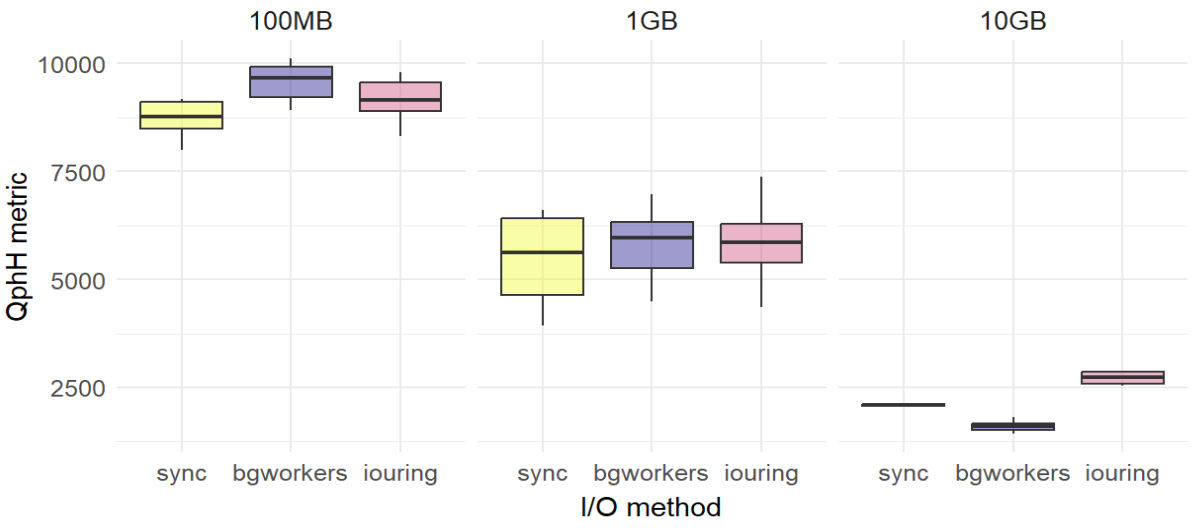
\includegraphics[width=\columnwidth]{images/data-all-gbs2.png}
    \caption{Comparison of QphH performance across I/O methods and database sizes (100MB, 1GB, 10GB). The performance degradation with increasing database size and the changing relative performance of I/O methods are clearly visible.}
    \label{fig:all_sizes}
\end{figure}

\begin{figure}[htbp]
    \centering 
    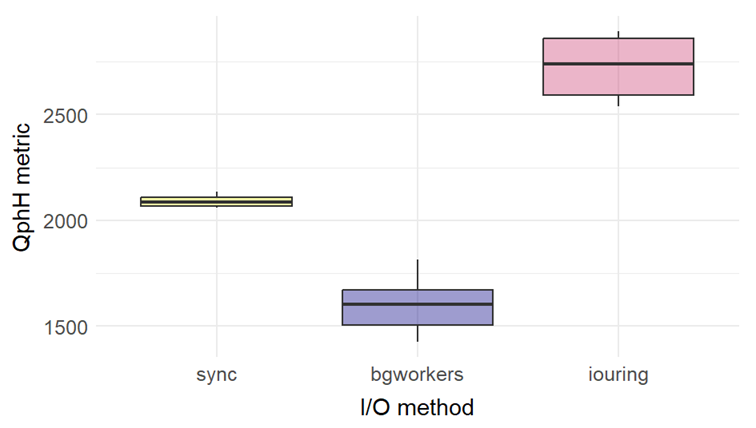
\includegraphics[width=0.8\columnwidth]{images/10-gb2.png}
    \caption{Detailed view of QphH performance at 10 GB database size, showing the clear performance hierarchy: \texttt{io\_uring} \textgreater \texttt{sync} \textgreater \texttt{bgworkers}.}
    \label{fig:10gb_detail}
\end{figure}

The superior performance of \textbf{io\_uring} aligns with its theoretical advantages: efficient system call batching, minimal context switching, and true asynchronous operation allowing the CPU to continue working while I/O requests are in flight. This architecture effectively masked I/O latency, leading to the highest throughput. It is particularly noteworthy that the \textbf{bgworkers} performed the worst at this scale, as clearly visible in \ref{fig:10gb_detail}. This suggests that the synchronous, multi-threaded approach of the background workers may introduce coordination overhead or contention that outweighs its parallel benefits under heavy I/O load. This may be interesting to study in future iteration. The fact that the single-threaded \textbf{sync} outperformed the \textbf{bgworkers} indicates that a streamlined synchronous approach can be more efficient than multiple synchronous threads contending for resources when the system is severely I/O-bound.


While this study focused specifically on PostgreSQL, the findings have broader implications for relational database design. The performance patterns observed suggest that other database systems implementing similar mechanisms (such as MySQL's \texttt{innodb\_use\_native\_aio} or Oracle's Direct NFS) might exhibit comparable behavior. Future work could extend this analysis to cross-platform comparisons.

Additional investigation is needed to further explore the performance boundaries of these I/O methods. A primary lead would be to test with significantly larger database sizes (e.g., 100 GB or 1 TB), where the working set vastly exceeds the available buffer cache and the system becomes profoundly I/O-bound.
We hypothesize that the performance advantages of \texttt{io\_uring}, in particular, would be even more pronounced under these extreme conditions. Additionally, the poor performance of the background worker method at the 10 GB scale could indicates a need for parameter tuning. A systematic study varying the number of background I/O workers is essential to identify if the default configuration was suboptimal for our test environment and to find the optimal parallelism level for different hardware and data scales.


\section*{Acknowledgment}

This research was supported by \ifanonymous [Anonymized entities]\else the School of Computer Science and Informatics (ECCI), and the Center for Research in Information and Communication Technologies (CITIC), both of the University of Costa Rica (UCR)\fi.

\ifanonymous
We would like to thank a colleague for his valuable contributions to the initial conceptualization and foundational work of this project.
\else
We would like to thank Milton Sojo-Córdoba of \textit{ECCI}, \textit{Universidad de Costa Rica} for his valuable contributions to the initial conceptualization and foundational work of this project.
\fi


The following AI tools were used in the preparation of this article: Grammarly, Google Translate, and Overleaf's AI-powered language tools for spellchecking and wording suggestions.

\begin{comment}
    This research was supported by the School of Computer Science and Informatics (ECCI), 
    and the Center for Research in Information and Communication Technologies (CITIC), 
    both of the University of Costa Rica (UCR).
    We would like to thank Professor Allan Berrocal (ECCI) for allowing us to use 
    his Overleaf instance for this work.
\end{comment}

% Data availability section (appears in both versions)
\section*{Open Research Data}
The code and data supporting this study are available in GitHub~\ifanonymous\cite{analysis_async_db_2025_anonymous}\else\cite{analysis_async_db_2025}\fi.

%} IDO Sobraba esta llave?

\begin{balance} %IDO
    
\bibliographystyle{IEEEtran}
\bibliography{references.bib}

\end{balance} %IDO

\end{document}
